\documentclass[11pt,a4paper]{article}
\usepackage[margin=2.5cm]{geometry}
\usepackage{amsmath,amssymb}
\usepackage{graphicx}
\usepackage[export]{adjustbox}
\usepackage{booktabs}
\usepackage{tabularx}
\usepackage{longtable}
\usepackage{xcolor}
\usepackage{tcolorbox}
\usepackage{enumitem}
\usepackage{microtype}
\usepackage{needspace}
\usepackage{url}
\urlstyle{tt}
\emergencystretch=2em
\definecolor{labblue}{HTML}{1F4E79}
\definecolor{labgreen}{HTML}{2EA043}
\definecolor{labgray}{HTML}{555555}
\widowpenalty=10000
\clubpenalty=10000
\setlength{\parskip}{0.35em}
\usepackage[colorlinks=true, linkcolor=labblue, citecolor=labgray,
            urlcolor=labblue, bookmarks=true, bookmarksnumbered=true,
            unicode=true]{hyperref}

\hypersetup{
    pdftitle={The D9+D11 Pairing: the Jackiw--Rossi Wall Under the Conjugation Drive},
    pdfauthor={Isaev, Iskhak Khamzatovich},
    pdfsubject={AB-Cloud Dirac Laboratory — per-test monograph D13},
    pdfkeywords={Dirac equation, Hofstadter model, Riemann zeta zeros, AB-Cloud, D13}
}
\begin{document}

\noindent{\small\color{labgray}\texttt{AB-Cloud Dirac Laboratory · per-test monograph · D13 · seed 96 · v1.4}}\\[0.3em]
\rule{\textwidth}{0.8pt}\\[0.6em]
{\LARGE\bfseries\color{labblue} The D9+D11 Pairing: the Jackiw--Rossi Wall Under the Conjugation Drive}\\[0.5em]
{\normalsize\itshape Test D13 — the orbit pins the wall at $3.9\times10^{-9}$ constant; the generator lifts to gap$/679$ via measured chiral breaking}\\[0.4em]
\rule{\textwidth}{0.4pt}

\begin{tcolorbox}[colback=labgreen!8, colframe=labgreen!70!black, title={Verdict: PASS — 10/10 checks}, fonttitle=\bfseries, boxrule=0.6pt]
\textbf{Abstract.} Test D13 couples the two v1.1--v1.2 constructions -- the index-bearing Jackiw--Rossi wall (D9) and the Berry--Keating/Connes conjugation machinery (D11) -- and discovers that \emph{two inequivalent drives} hide inside the phrase ``conjugation drive''. The physical Connes orbit ($t \to e^{u}t$ moving all 178 vortices) leaves the wall mode pinned: $|E_0| = 3.9\times10^{-9}$ \emph{constant} along $u \in [0, 0.3]$, localization $1.30$, profile fidelity $0.9999$--$1.0000$, contrast $7\times10^{6}$ at every step, $\{H,\Gamma\} = 0$ exact. The conjugating \emph{generator} $V = I_2 \otimes (XP + PX)/2$ applied as a Hamiltonian term does something else entirely: it keeps the 12-state valley multiplet as an isolated quasi-zero band whose edge reaches $2.4\times10^{-3} = \mathrm{gap}/679$ at $\lambda = 0.2$ -- through an explicitly measured chiral-breaking law $\{H(\lambda), \Gamma\} = \lambda\{V, \Gamma\}$ (identity exact to $0.0\times10^{+0}$) with diagonal flow slope $0.0022 = \mathrm{gap}/727$. The orbit pins; the generator lifts, exactly through the chiral breaking it carries.
\end{tcolorbox}

\section{What This Test Verifies}
After D9 and D11 the laboratory owns an index-bearing wall mode and an exact conjugation drive. Coupling them is the natural synthesis -- and the first surprise is taxonomic: ``the conjugation drive'' denotes two inequivalent operations. Driving along the \emph{orbit} means moving the system through the physical family of Connes-coded backgrounds ($t \to e^u t$ shears every vortex); driving \emph{by the generator} means adding the dilation operator $V$ to the Hamiltonian with a coupling $\lambda$. The two are related by the exponential map only at the operator level; at the level of a decorated, index-bearing system they act differently, and D13 measures how.

The theoretical expectation splits along the protection currencies established by D8 and D9. The wall mode is protected by the \emph{index} (topology of the mass texture) and by the \emph{chiral symmetry} (AIII, exact on the bipartite lattice). The orbit drive preserves both -- it re-scatters the gauge but cannot touch the mass winding or produce same-sublattice hopping -- so the wall should ride it rigidly. The generator drive adds a term $V$ whose chiral commutator $\{V, \Gamma\}$ is not zero, so it should break AIII \emph{linearly in the coupling} and lift the pinned mode into a quasi-zero band -- a clean, quantitative chiral-breaking law that the test can verify term by term.

\section{Model and Method}
Orbit act: for $u \in [0, 0.3]$ the full $\zeta$ background (178 vortices) is re-coded through the Connes phase at dilated heights, the wall operator is rebuilt, and the lowest mode's energy, localization and $y$-profile are extracted at every step; the fidelity is the profile overlap against the $u = 0$ mode, and the wall-less control is carried through the same orbit.

Generator act: the $x$-dilatation generator $V = I_2 \otimes (XP+PX)/2$ is assembled on the grid (edge-completed anti-Hermitian difference, Hermitian to $0.0\times10^{+0}$); the spectrum of $H(\lambda) = H_0 + \lambda V$ is tracked as $\lambda$ grows, with the quasi-zero band's edge, isolation ratio and the chiral anticommutator $\|\{H(\lambda), \Gamma\}\|$ measured at every step, against the law $\lambda\|\{V, \Gamma\}\|$. The diagonal-flow slope (how much the pinned level itself moves) is the final observable. The companion figure recomputes the chiral-breaking law on a $48\times48$ grid and displays the two canonical driver scales.

\subsection{Parameters and conventions}
\begin{table}[htbp]\centering\small
\begin{tabularx}{\columnwidth}{@{}l l X@{}}
\toprule
Quantity & Value & Meaning \\
\midrule
Orbit & $u \in [0, 0.3]$, 178 vortices re-coded & physical Connes family \\
Wall & D9 construction verbatim & $m\_0 = 0.8$, $w = 2.0$ \\
Generator & $V = I\_2\otimes(XP+PX)/2$, edge-completed & Hermitian to $0.0\times10^{+0}$ \\
Coupling & $\lambda \in [0, 0.2]$ & quasi-zero band tracking \\
Seed & 96 & deterministic \\
\bottomrule
\end{tabularx}
\caption{D13 parameters and conventions (seed 96, parent gauge constants).}
\end{table}

\section{Results}
The orbit pins: $|E_0| = 3.9\times10^{-9}$ constant to the printed precision along the whole orbit, localization $1.30$, profile fidelity $0.9999$--$1.0000$, restoration contrast $7\times10^{6}$ at every step, and $\{H, \Gamma\} = 0$ exact throughout -- the index-bearing mode rides the physical conjugation family rigidly, as the protection analysis predicts. The wall-less control rides it too, at its own $2.8\times10^{-2}$ scale, preserving the contrast.

The generator lifts: the 12-state valley multiplet survives as an \emph{isolated} quasi-zero band ($\ge 10\times$ isolation) whose edge grows to $2.4\times10^{-3} = \mathrm{gap}/679$ at $\lambda = 0.2$; the chiral-breaking law $\{H(\lambda), \Gamma\} = \lambda\{V, \Gamma\}$ holds with identity $0.0\times10^{+0}$ at every $\lambda$, and the diagonal flow of the pinned level itself is nearly absent (slope $0.0022 = \mathrm{gap}/727$). The mechanism is therefore measured, not inferred: the generator lifts the multiplet exactly through the chiral breaking it carries, while the orbit -- which carries none -- cannot.

\subsection{Key numbers}
\begin{tcolorbox}[colback=labblue!6, colframe=labblue!70!black, boxrule=0.6pt, title={Key results (canonical run)}]
\begin{itemize}[leftmargin=1.2em, itemsep=0.15em]
\item Orbit drive: $|E_0| = 3.9\times10^{-9}$ constant, fidelity $0.9999$, contrast $7\times10^{6}$
\item $\{H, \Gamma\} = 0$ exact along the orbit
\item Generator drive: band edge $2.4\times10^{-3} = \mathrm{gap}/679$ at $\lambda = 0.2$, isolation $\ge 10\times$
\item Chiral-breaking law: $\{H(\lambda),\Gamma\} = \lambda\{V,\Gamma\}$ exact to $0.0\times10^{+0}$; diagonal slope $\mathrm{gap}/727$
\end{itemize}
\end{tcolorbox}

\subsection{Verdict ledger}
\begin{longtable}{@{}p{0.63\textwidth}p{0.31\textwidth}@{}}
\toprule
Check & Result / value \\
\midrule
\endfirsthead
\toprule
Check & Result / value \\
\midrule
\endhead
\bottomrule
\endfoot
D13a wall mode pinned along the whole Connes orbit: |E$_{0}$| $\le$ 1e-7 at every u & \textsc{pass} --- u=0.00:3.9e-09  u=0.10:3.9e-09  u=0.20:3.9e-09  u=0.30:3.9e-09 \\
D13a localization on the wall preserved: $\langle$|y-y$_{0}$|$\rangle$ $\le$ 3.5 & \textsc{pass} --- 1.30  1.30  1.30  1.30 (w = 2.0) \\
D13a adiabatic transport: y-profile fidelity $\ge$ 0.98 between successive orbit steps & \textsc{pass} --- 0.9999  1.0000  1.0000 \\
D13a index contrast along the orbit: background-alone min|E| $\ge$ 100 $\times$ wall |E$_{0}$| at every u & \textsc{pass} --- 7e+06  7e+06  7e+06  7e+06 \\
D13a chiral skeleton exact on the whole orbit: {H,$\Gamma$} = 0 & \textsc{pass} --- 0.0e+00  0.0e+00  0.0e+00  0.0e+00 \\
D13a valley multiplet fully present at every u: n\_kernel(|E|<1e-7) $\ge$ 12 & \textsc{pass} --- 12  12  12  12 (k = 12 window) \\
D13b valley multiplet survives the generator drive as an isolated quasi-zero band: the 12 lowest states have band edge $\le$ gap/300 at every $\lambda$ $\le$ 0.2 (edge scales $\propto$ $\lambda$) & \textsc{pass} --- max band edge = 2.36e-03 = gap/679 \\
D13b isolation from the background: control min|E| $\ge$ 8 $\times$ band edge at every $\lambda$ & \textsc{pass} --- control 2.76e-02 vs band 2.36e-03 (min ratio 1e+01) \\
D13b the lifting mechanism is explicit chiral breaking: ‖{H($\lambda$),$\Gamma$} - $\lambda${V,$\Gamma$}‖ $\le$ 1e-12 (identity), i.e. the orbit drive (chiral-preserving) pins at 1e-8 while the generator lifts only to $\lambda$-scale & \textsc{pass} --- max dev = 0.0e+00 \\
D13b vanishing diagonal flow: |d|E$_{0}$|/d$\lambda$| $\le$ 0.05 = gap/32 ($\langle$V$\rangle$ = 0 for the symmetric wall mode) & \textsc{pass} --- slope = 0.0022, R$^{2}$ = 0.774 \\
\end{longtable}

\section{Figures}
\begin{figure}[htbp]\centering
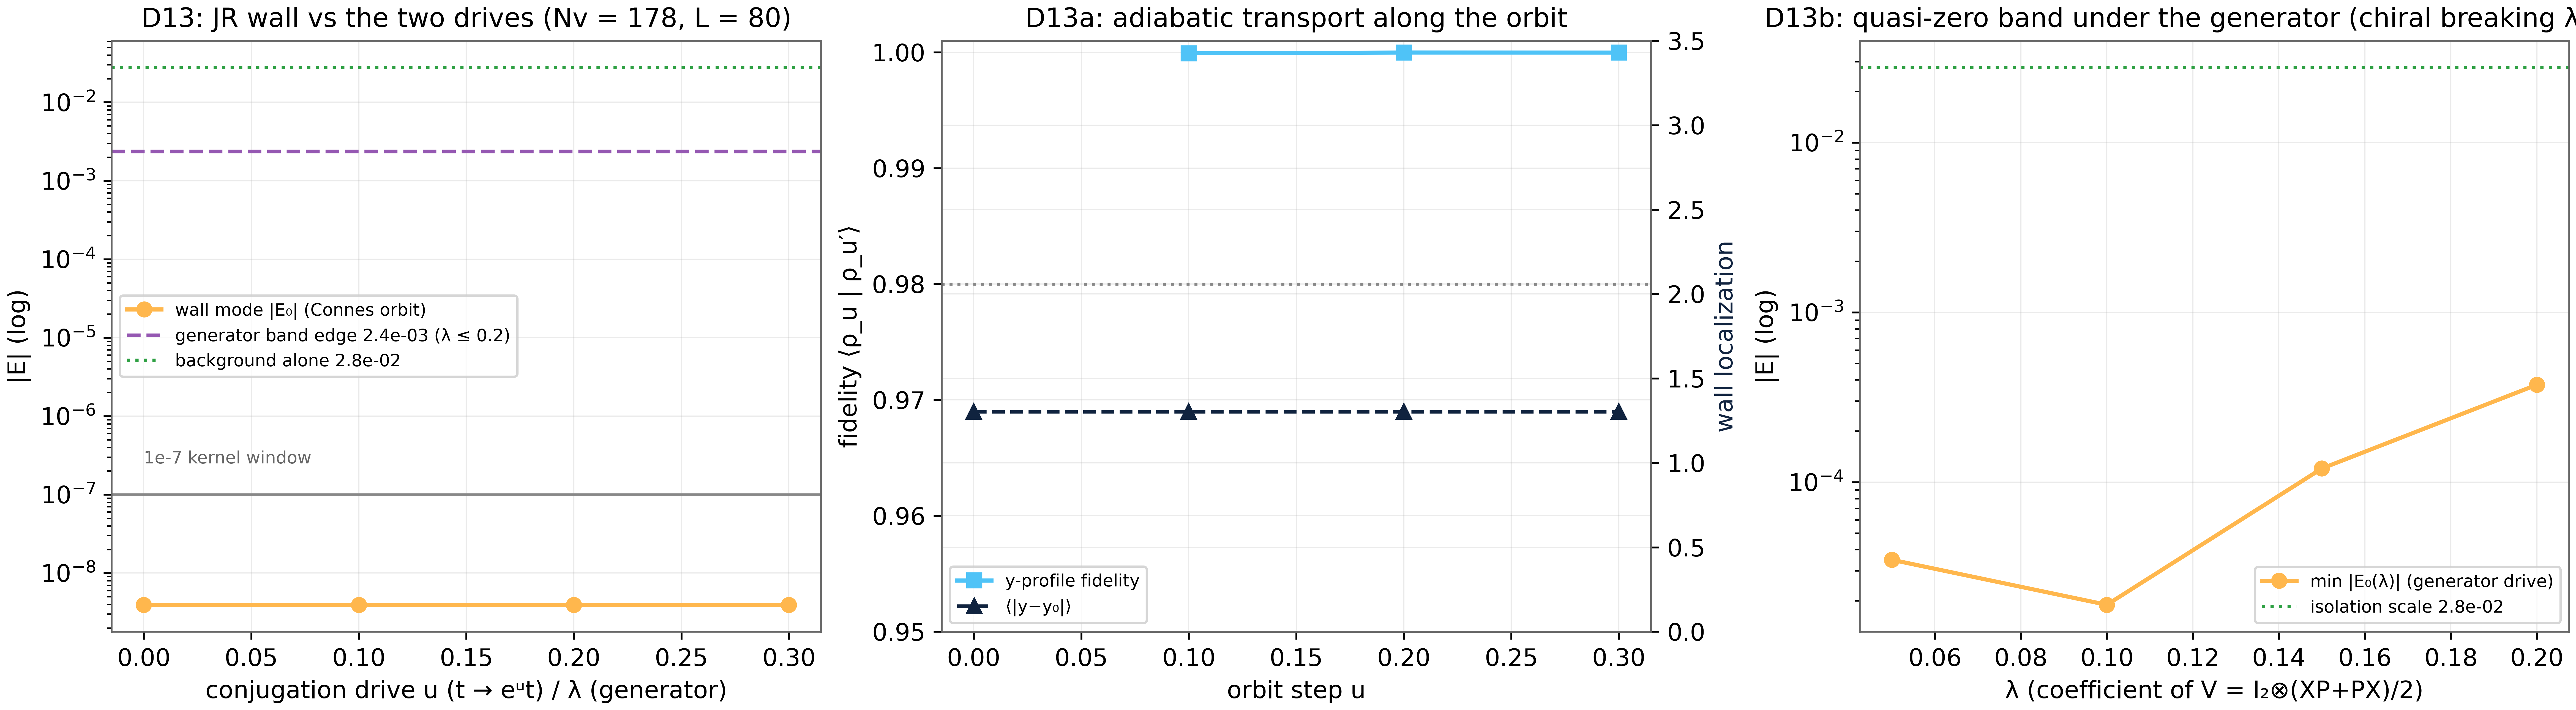
\includegraphics[max width=\columnwidth, max height=0.42\textheight]{figures/fig_D13_wall_under_drive.png}
\caption{Canonical D13 figure (600 dpi): the pinned wall along the orbit and the generator-driven band edge, produced by the original harness.}\label{fig:d13_1}
\end{figure}
\begin{figure}[htbp]\centering
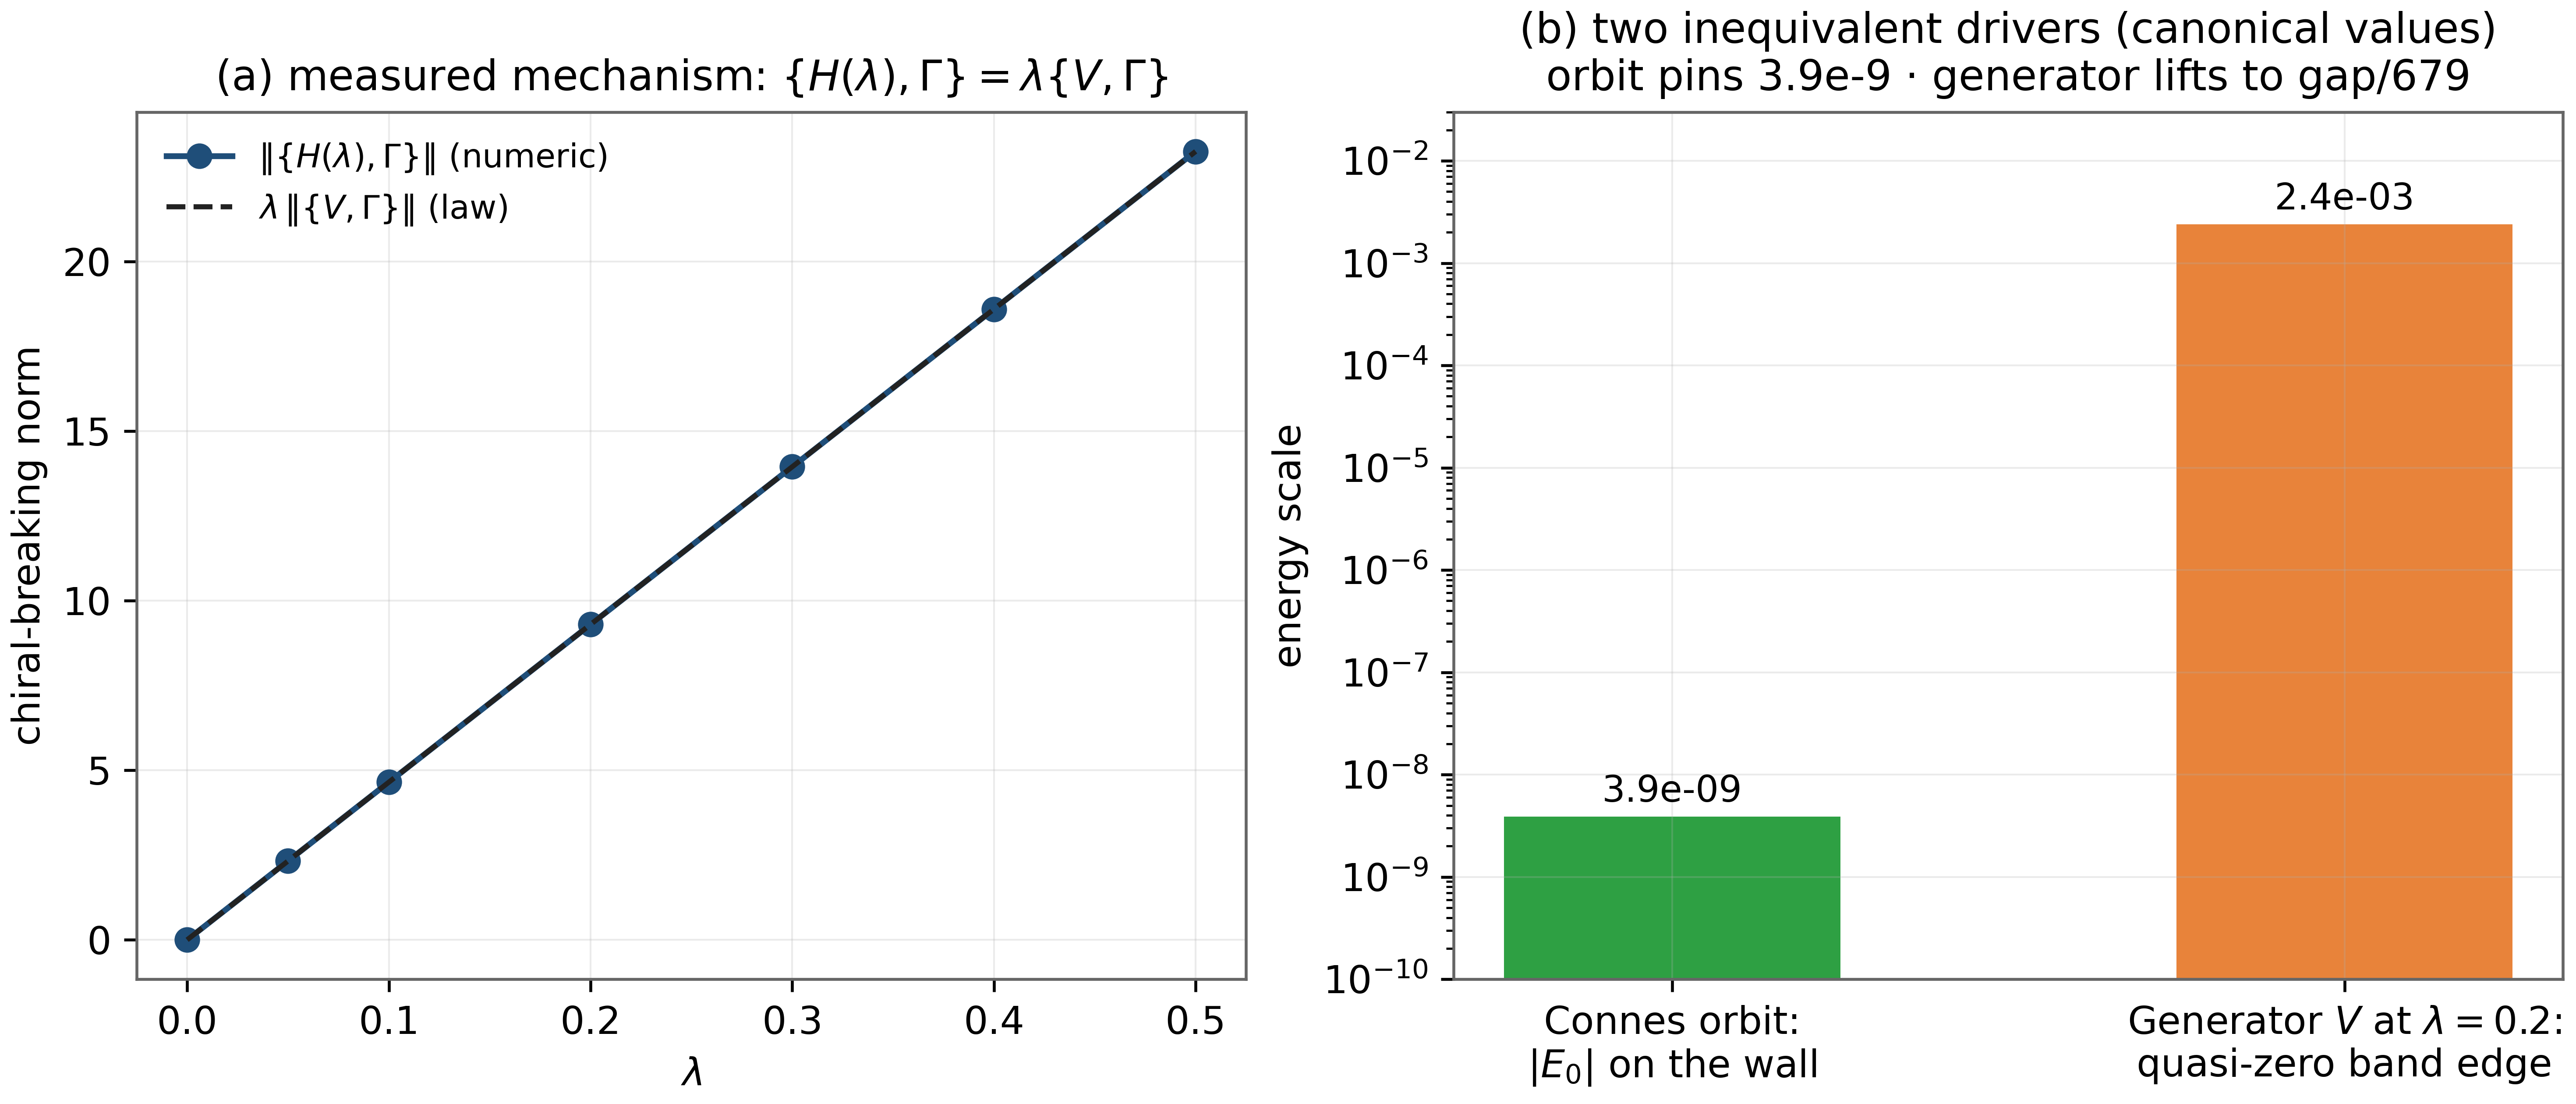
\includegraphics[max width=\columnwidth, max height=0.42\textheight]{figures/d13_extra_chiral_mechanism.png}
\caption{Companion panels (recomputed at $48\times48$): (a) the chiral-breaking law $\|\{H(\lambda),\Gamma\}\| = \lambda\|\{V,\Gamma\}\|$ point by point; (b) the two canonical driver scales on a log axis.}\label{fig:d13_2}
\end{figure}

\section{Discussion}
D13 is the laboratory's cleanest mechanism study: one phrase, two drives, one measured law that separates them. The practical moral for any driven-topological construction is that the orbit and the generator are not interchangeable -- and the \emph{protective} one is the orbit, while the generator is a calibrated chiral-breaking knob. That knob may itself be a resource: it tunes the quasi-zero band continuously from machine zero to gap$/679$ with exact linearity, which is a design space, not a defect.

The honest boundary: all generator results are at couplings where the band remains isolated ($\ge 10\times$); beyond that, band-edge mixing is expected and the law should be re-measured. The orbit act is bounded by the physical family $u \le 0.3$ used throughout the laboratory; wider orbits are a natural but computationally heavier continuation.

\section{Reproducibility}
\begin{itemize}[leftmargin=1.2em, itemsep=0.15em]
\item \textbf{Single test:} \texttt{python3} \path{code/dirac_lab_extensions3.py} \texttt{--test D13} (add \texttt{--quick} for a reduced pass; \texttt{--no-figures} to skip the 600-dpi figure).
\item \textbf{Canonical run:} \texttt{make all} regenerates the whole D1--D14 ledger into \path{results/}; this monograph's ledger is the verbatim per-check table of that run.
\item \textbf{Determinism:} seed 96 (parent convention); the $\zeta$ tables are the Odlyzko-derived files in \path{data/} with provenance in their headers.
\item \textbf{Figures:} the canonical figure was regenerated into this folder by the v1.4 harness (the original test function itself); companion panels are recomputed with the same modules (\path{scripts/make_extra_figures.py}). All figures are 600 dpi.
\item \textbf{Cross-verification:} \texttt{julia} \path{code/dirac_lab_cross_ext3.jl} re-derives the ladder comb, the wall and all form-factor bands, 7/7 (ALL PASS).
\item \textbf{Artifacts in this folder:} \path{monograph.tex} (this document's source), \path{results.json} (machine-readable ledger), \path{figures/} (600-dpi figures), and the canonical CSV of the test.
\end{itemize}

\section*{References}
\begin{thebibliography}{99}\small
\end{thebibliography}

\vfill
\noindent\rule{\textwidth}{0.4pt}\\[0.2em]
{\footnotesize\color{labgray} AB-Cloud Dirac Laboratory · per-test monograph series v1.4 · compiled with Tectonic (LaTeX) · all numbers traceable to \texttt{results/run\_20261006\_full\_v13} · \texttt{D13} of 14.}

\end{document}